\chapter{Mecánica de juego}
%=========================================================
	\section{Cámara}
El juego se manejara en 2D, desde una perspectiva lateral. La cámara será ortogonal y seguirá al jugador en sus movimientos sobre el eje x y y, existiendo algunas secciones de los niveles limites en cuanto a su desplazamiento, tal como muestra la figura \ref{fig:Camara}. 

\begin{figure}
  \centering
  \subfigure[Seguimiento horizontal]{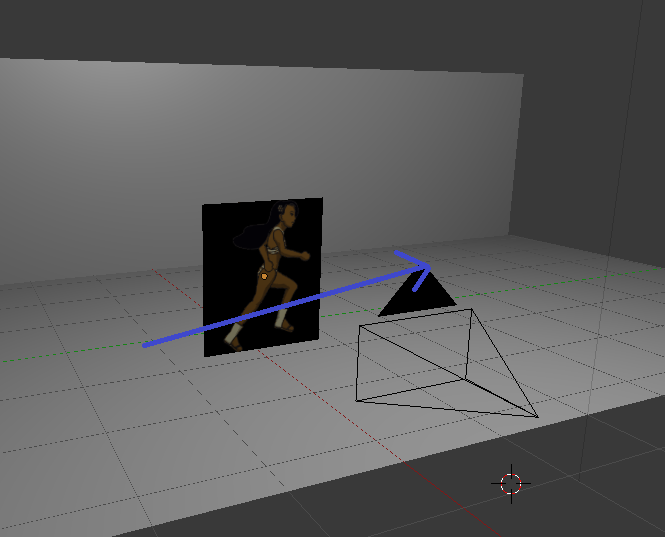
\includegraphics[width=0.7 \textwidth]{Imagenes/camara01}}
   \subfigure[Seguimiento vertical.]{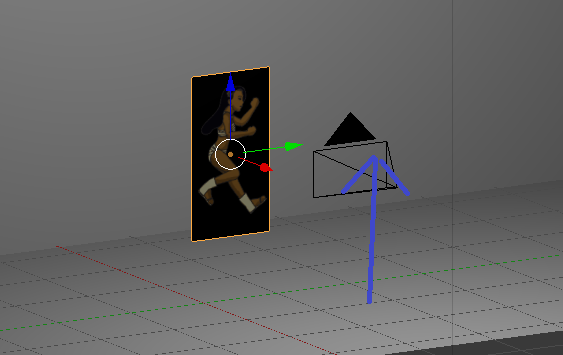
\includegraphics[width=0.7 \textwidth]{Imagenes/camara02}}
  \caption{La cámara seguirá la posición del jugador en el eje x y y.}
 %=========================================================
  \label{fig:Camara}
\end{figure} 
%=========================================================
	\section{Periféricos}
	Patalla táctil.
%=========================================================
	\section{Controles}
	Del lado izquierdo inferior de la pantalla existirán cuatro botones: dos botones de desplazamiento, uno de salto y otro de disparo.Todos estos botones son de forma circular y en conjunto ocupan un cuarto de la pantalla (ver figura \ref{fig:Controles}). A continuación se describirá cada botón y su funcionamiento.
	\begin{itemize}
		\item \textbf{Botón moverse derecha:} Botón cuyo icono es una flecha apuntando hacia la derecha. Permite al personaje jugable desplazarse hacia la derecha.
		\item \textbf{Botón moverse izquierda:} Botón cuyo icono es una flecha apuntando hacia la izquierda. Permite al personaje jugable desplazarse hacia la izquierda.
		\item \textbf{Botón disparar:} Botón cuyo icono es una flama girada noventa grados en sentido contrario de las manecillas del reloj. La acción de este botón depende de la cantidad de tonalli del personaje jugable. Cuando ésta es mayor a cero, el jugador dispara esferas de energía que desaparecen después de determinado tiempo. Estas esferas de energía pueden efectuar una cantidad de daño en los enemigos de cada nivel pero no tienen efecto sobre los obstáculos. Cada disparo decrementa la cantidad de tonalli total de manera constante, cuando ésta llega a cero el jugador no podrá realizar ningún disparo hasta que se recargue la barra de cantidad de tonalli(la cual tiene un tiempo de recarga automática una vez que llega a cero) o toque el item de flor de vainilla.
		\item \textbf{Botón saltar:} El icono de este botón es una flecha que apunta hacia arriba. Este botón solamente se puede accionar dos veces seguidas, es decir permite hacer de manera consecutiva dos saltos.  
	\end{itemize}
	\begin{figure}
  \centering
  \subfigure[Acción del botón de moverse derecha.]{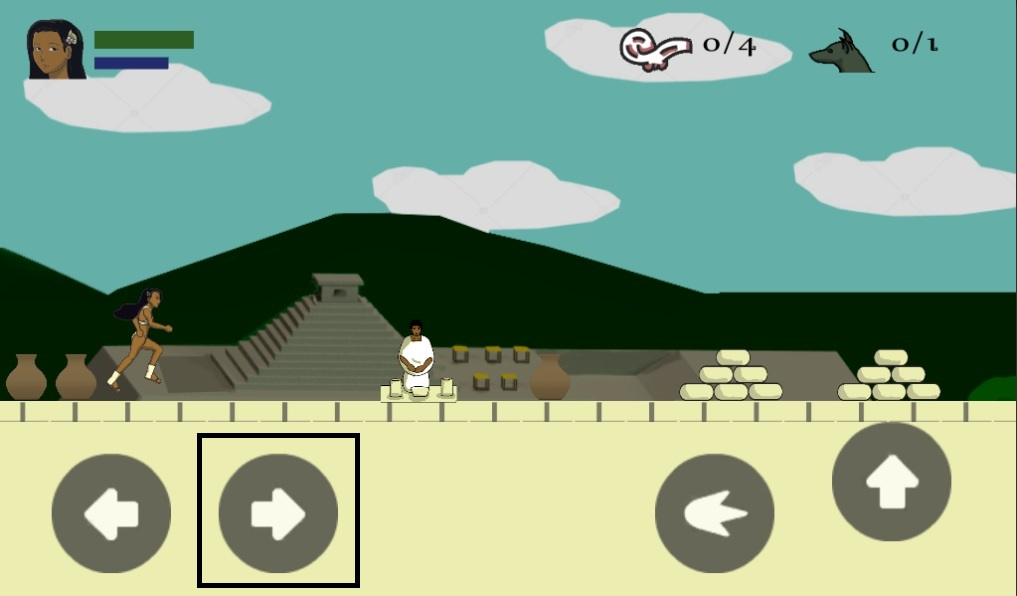
\includegraphics[width=0.45 \textwidth]{Imagenes/ControlCorrerDerGUI}}
   \subfigure[Acción del botón de moverse izquierda.]{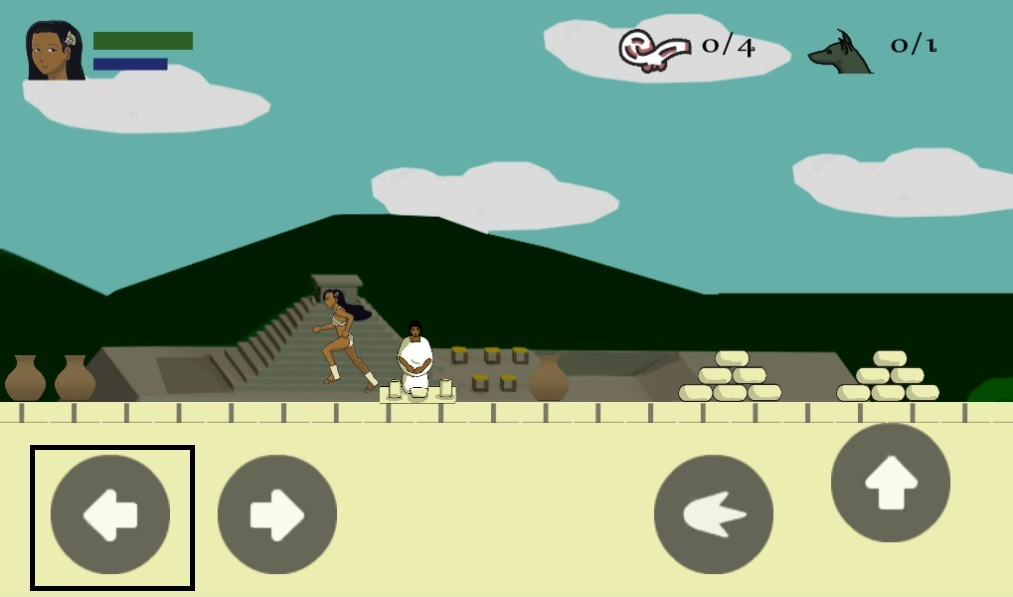
\includegraphics[width=0.45 \textwidth]{Imagenes/ControlCorrerIzq}}
   \subfigure[Acción del botón de disparar.]{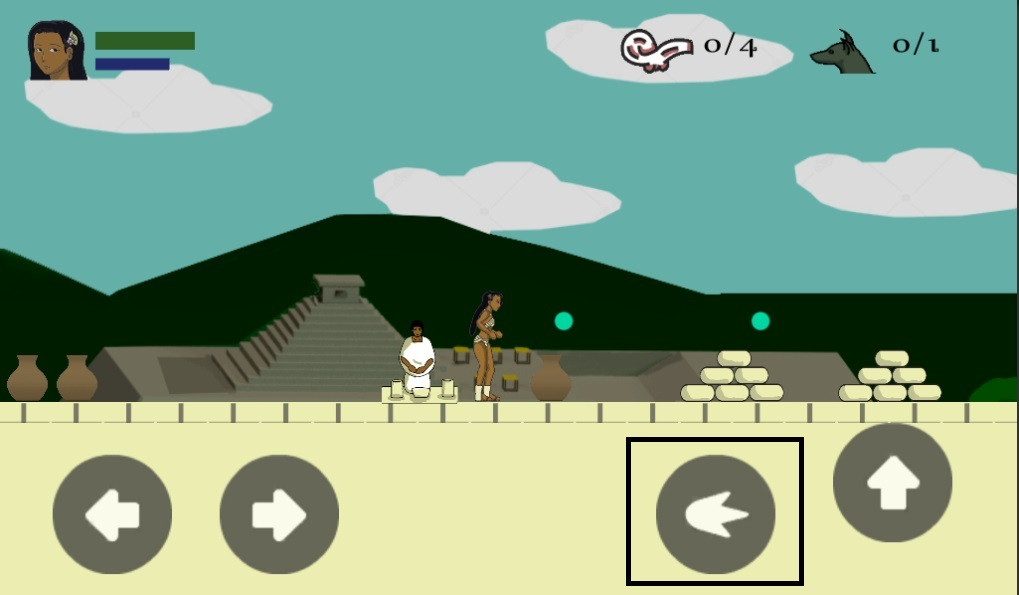
\includegraphics[width=0.45 \textwidth]{Imagenes/Controldispara}}
   \subfigure[Acción del botón de saltar.]{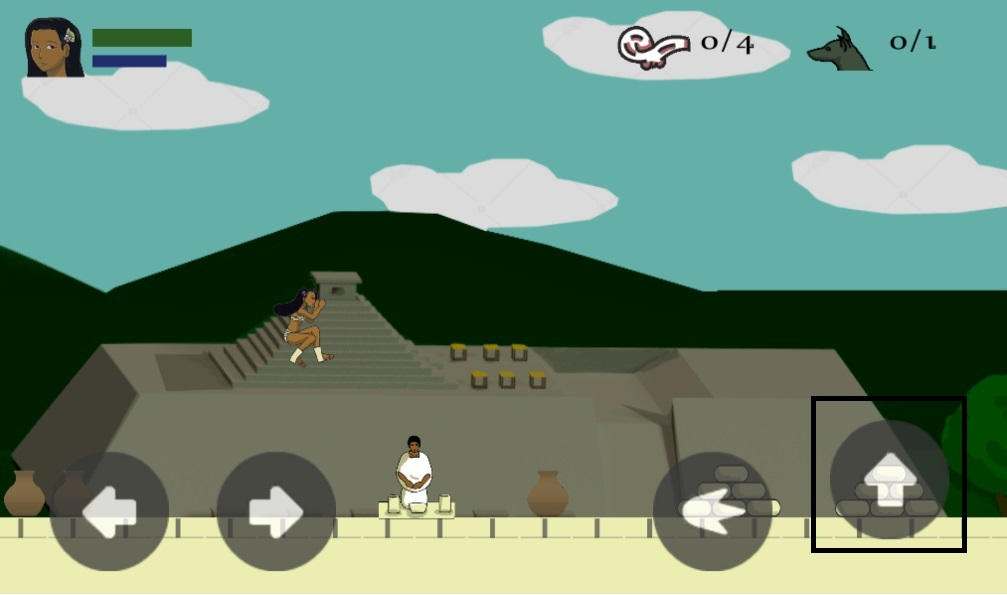
\includegraphics[width=0.45 \textwidth]{Imagenes/ControlSalta}}
  \caption{Acciones que desencadena cada botón.}
  \label{fig:Controles}
\end{figure} 
%=========================================================
	\section{Guardar/Cargar}
	%---------------------------------------------------------
\subsection{Guardar}
Dentro del juego existen dos tipos de guardado en el juego: el guardado automático y el checkpoint. 
\begin{itemize}
\item \textbf{Guardado automático}: 
Este tipo de guardado se realizará cuando el jugador haya completado un nivel. En este tipo de guardado se almacenara información como los niveles y cinemáticas disponibles, y las estadísticas del jugador(cantidad de vida, cantidad de tonalli y capacidad de daño). 
\item \textbf{Checkpoint}: 
Este tipo de guardado almacena la posición del jugador en un punto determinado del nivel. Los puntos de checkpoint son representados dentro del juego con el objeto Tecolote. El checkpoint se activará cuando el jugador colisione con el objeto tecolote( ver apartado \ref{per:tecolote}) . Este tipo de guardado es efectivo mientras el jugador se mantenga dentro del nivel y la información almacenada se perderá si el jugador abandona la partida.
Los puntos de checkpoint están disponibles a partir del segundo nivel del juego y hasta el noveno nivel. La cantidad de checkpoints dependerá del nivel, pudiendo haber de dos a cuatro checkpoints. 
\end{itemize}
%---------------------------------------------------------
\subsection{Cargar}
Dentro del juego existen dos tipos de carga en el juego: carga automática y el checkpoint. 
\begin{itemize}
\item \textbf{Carga automática}: 
Este tipo de cargado se realizará cuando el jugador seleccione la opción de cargar partida desde la Interfaz 2.00(ver apartado \ref{inter:interfaz02})o cuando el jugador se encuentre en la interfaz 03 (ver apartado \ref{inter:interfaz03}). En este tipo de carga le permite al juego conocer el progreso del jugador, por lo que en esta carga el juego conocerá información como los niveles y cinemáticas disponibles, y las estadísticas del jugador (cantidad de vida, cantidad de tonalli y capacidad de daño). 
\item \textbf{Checkpoint}: 
Este tipo de carga permite que el jugador pueda aparecer en la posición del ultimo objeto Tecolote ( ver apartado \ref{per:tecolote}) con el que se haya colisionado dentro del juego una vez que el jugador haya muerto y no haya abandonado la partida. Cuando se carga la posición del jugador en el Checkpoint, el jugador recuperara al máximo la cantidad de vida y de tonalli que tenga disponible para ese nivel.
\end{itemize}
			
